\documentclass[9pt]{IEEEtran}

\usepackage[english]{babel}
\usepackage{graphicx}
\usepackage{epstopdf}
\usepackage{fancyhdr}
\usepackage{amsmath}
\usepackage{amsthm}
\usepackage{amssymb}
\usepackage{url}
\usepackage{array}
\usepackage{textcomp}
\usepackage{listings}
\usepackage{hyperref}
\usepackage{xcolor}
\usepackage{colortbl}
\usepackage{float}
\usepackage{gensymb}
\usepackage{longtable}
\usepackage{supertabular}
\usepackage{multicol}

\usepackage[utf8x]{inputenc}
\usepackage{caption}
\captionsetup[figure]{justification=centering}

\usepackage[T1]{fontenc}
\usepackage{lmodern}
\input{glyphtounicode}
\pdfgentounicode=1

\graphicspath{{./figures/}}
\DeclareGraphicsExtensions{.pdf,.png,.jpg,.eps}

% correct bad hyphenation here
\hyphenation{op-tical net-works semi-conduc-tor trig-gs}

% ============================================================================================

\title{\vspace{0ex} Mean Shift Tracking Algorithm}

\author{Aljaž Konec\vspace{-4.0ex}}

% ============================================================================================

\begin{document}

\maketitle

\section{Introduction}
In this report we present the implementation of the Mean Shift tracking algorithm. 
The algorithm uses a kernel density estimation to find the mode of a probability density function PDF.
In the context of tracking, the PDF represents the color distribution of the object to be tracked.
The algorithm iteratively shifts the kernel towards the mode of the PDF until convergence.
For the kernel density we use the Epachenik kernel for its simplicity and computational efficiency.
The report is split into two parts.
In the first part we describe and test mean shift mode seeking and in the second part we apply mode seeking for tracking and showcase the results on the VOT 2014 dataset.


\section{Mean Shift Mode Seeking}
Figure \ref{fig:mean_shift} shows the results of mean shift mode seeking on a synthetic image.
We test the algorithm with four different kernel sizes and multiple starting points.
For kernel size 15 it can be seen that some starting positions do not converge to the global maximum.
Increasing the kernel size to more than 31 completley negates this local convergance as the kernel is large enough to include the higher values of the global maximum.
\begin{figure}[h]
    \centering
    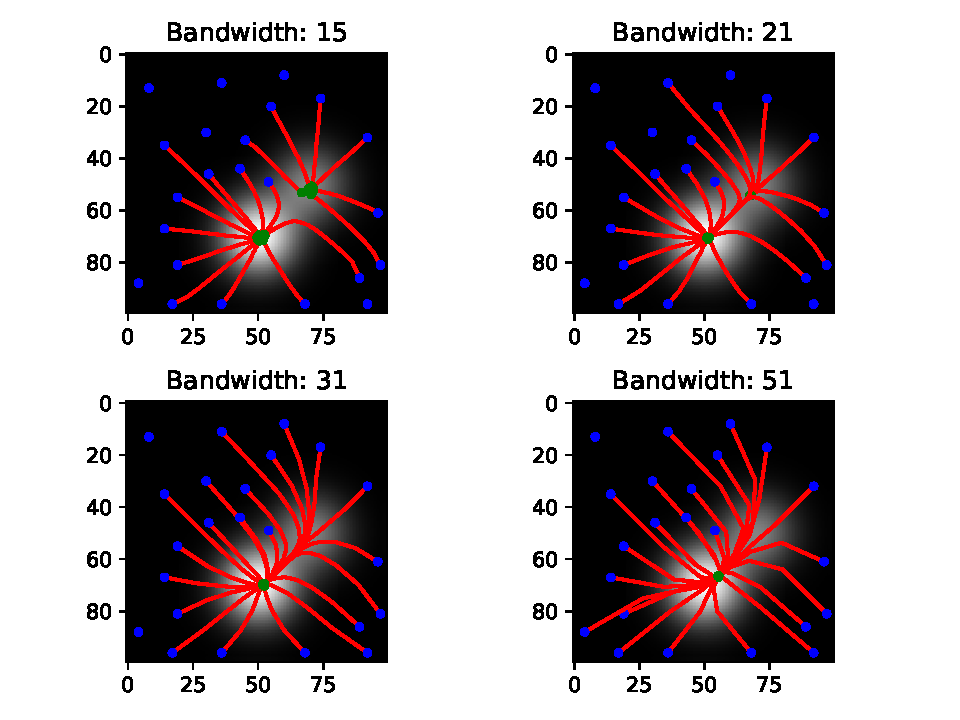
\includegraphics[width=1\columnwidth]{mean_shift.pdf}
    \caption{Mean shift mode seeking.}
    \label{fig:mean_shift}
\end{figure}
To improve convergance speed and accuracy we start decreasing the kernel size by 2 as soon as the length of the shift vector is smaller than 0.4 pixels.
We completley terminate the algorithm when the shift is smaller then 0.1 pixels.
Using these convergance criteria we get the following convergance speeds:
\begin{itemize}
    \item Kernel size 15: 17.0 iterations
    \item Kernel size 21: 17.5 iterations
    \item Kernel size 31: 13.7 iterations
    \item Kernel size 51: 12.3 iterations
\end{itemize}

\subsection{Mean Shift Mode seeking on custom sythetic image}
Figure \ref{fig:mean_shift_custom} shows the results of mean shift mode seeking on a custom synthetic image to show the robustness of the algorithm.
\begin{figure}[h]
    \centering
    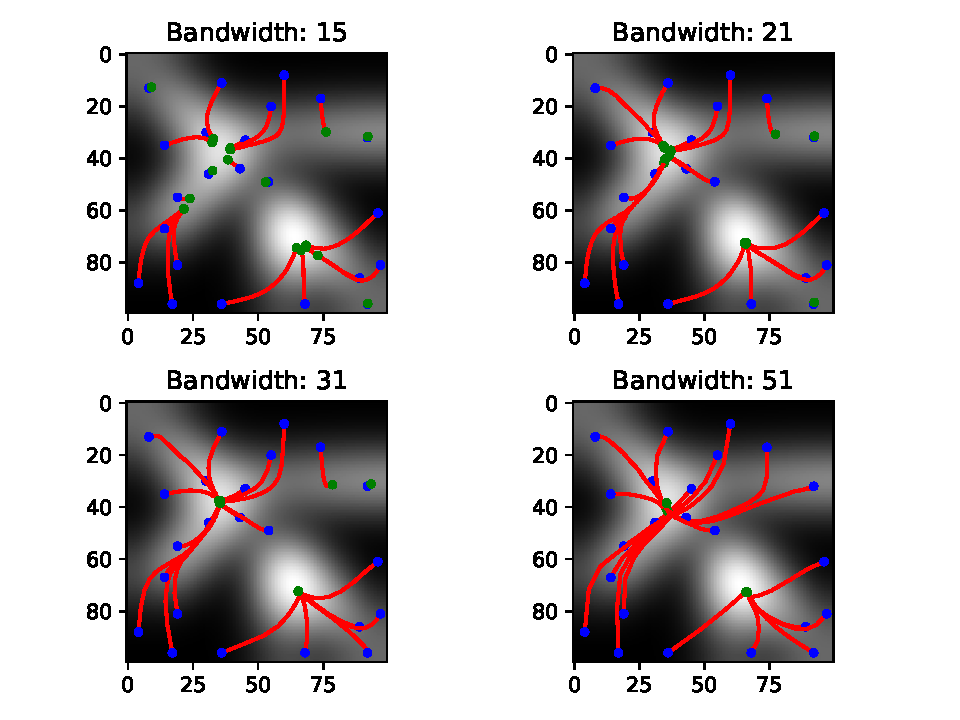
\includegraphics[width=1\columnwidth]{mean_shift_custom.pdf}
    \caption{Mean shift mode seeking on custom synthetic image.}
    \label{fig:mean_shift_custom}
\end{figure}
This case showcases how to small of an intial kernel size can lead to convergance in a local maximum.
For most of the starting positions, a kernel size of 15 is too small to converge to the global maximum.
Kernels with size 31 and 51 cover the appropriatly sized area and converge to acceptable maximums.
The paths from starting positions to the maximums are also longer beacause the of longer ridges which have to be traversed.
For this reasons the convergance speed is the following:
\begin{itemize}
    \item Kernel size 15: 23.3 iterations
    \item Kernel size 21: 28.4 iterations
    \item Kernel size 31: 23 iterations
    \item Kernel size 51: 25 iterations
\end{itemize}

\section[short]{Mean Shift Tracking}


\begin{figure}[h]
    \centering
    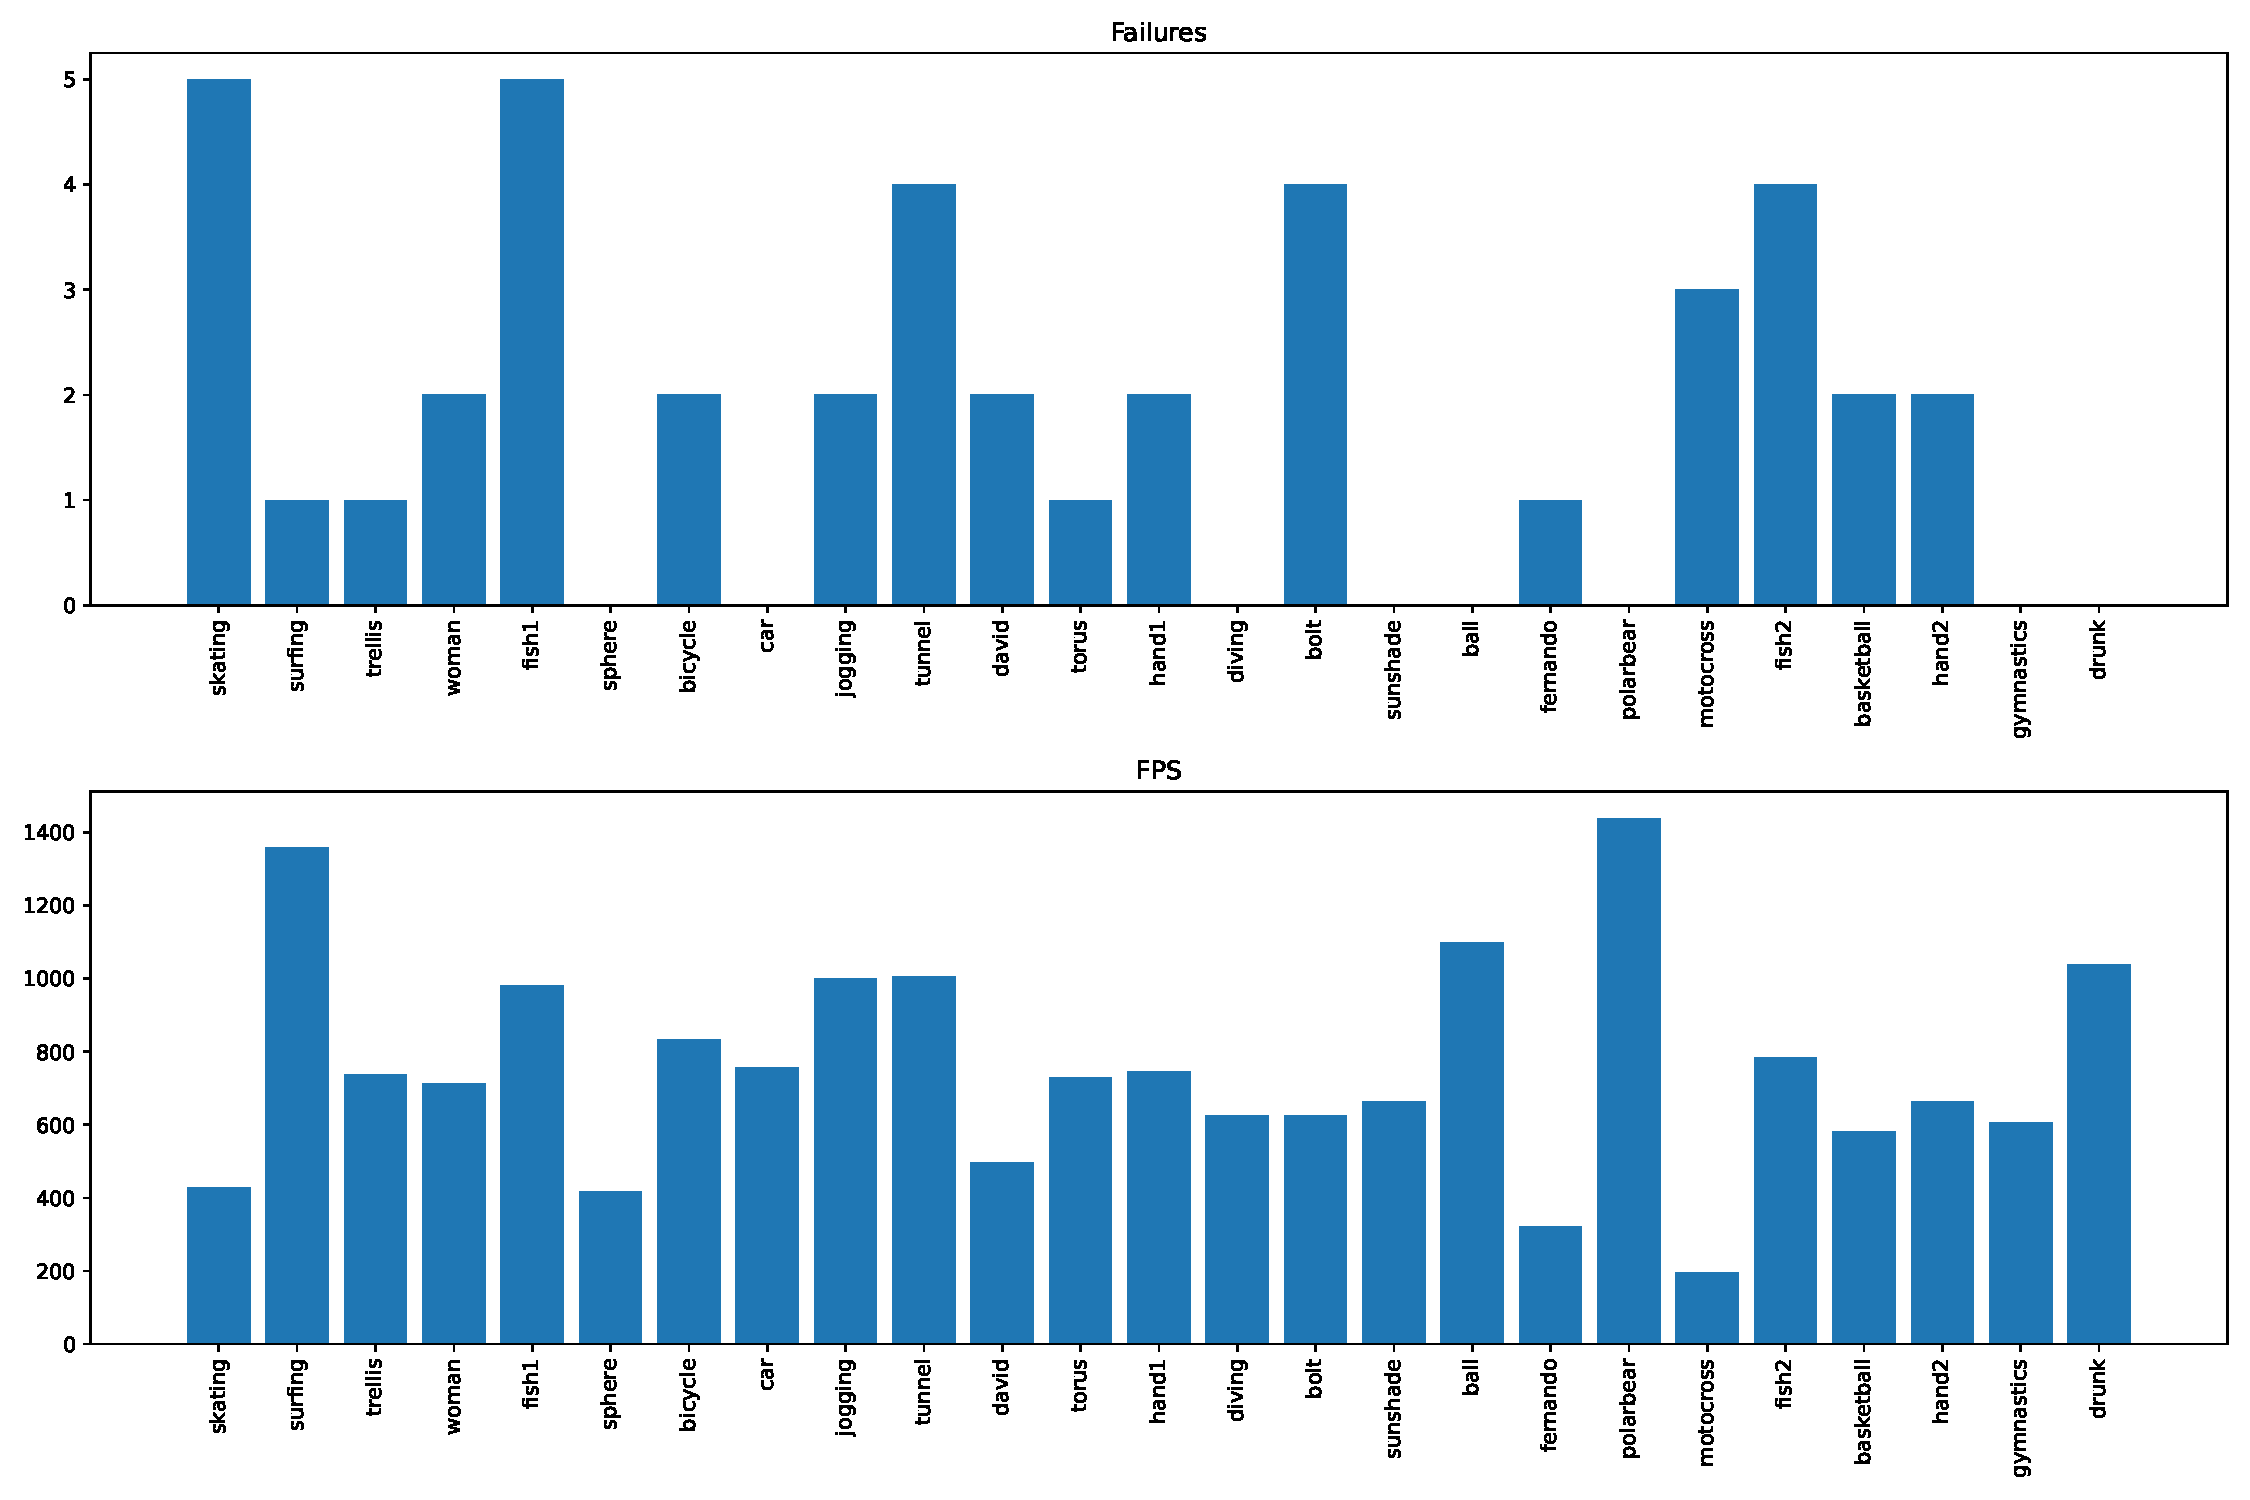
\includegraphics[width=1\columnwidth]{vot_performance.pdf}
    \caption{Mean shift tracking on VOT 2014 dataset.}
    \label{fig:mean_shift_tracking}
\end{figure}
We use the mean shift mode seeking algorithm to track an object in a video sequence.
The object is represented as histogram of the color distribution in the object region.
To find the object in the next frame we use the mean shift algorithm on a weighted quotient of target and candidate histograms.
When computing the quotient we add a small constant number $\epsilon$ to the denominator to avoid division by zero.
We repeat this process until the shift vector is smaller than 0.2 pixels or the number of iterations exceeds 50.
Figure \ref{fig:mean_shift_tracking} shows the results of the mean shift tracking algorithm on the VOT 2014 dataset.
Using the best performing parameters that we discuss in the following subsections we see that the tracker fails at most 5 times in a single video.
Combined, the tracker fails 42 times and in average achives a rate of 750 FPS, if we do not show the frames. 

\subsection*{Failure cases}
In this section we discuss failure cases of the mean shift tracking algorithm.
We focus on the following video sequences: bolt, skating, fish1 and tunnel.
Figure \ref{fig:failures} shows the failure cases of the mean shift tracking algorithm.
\begin{figure}[h]
    \centering
    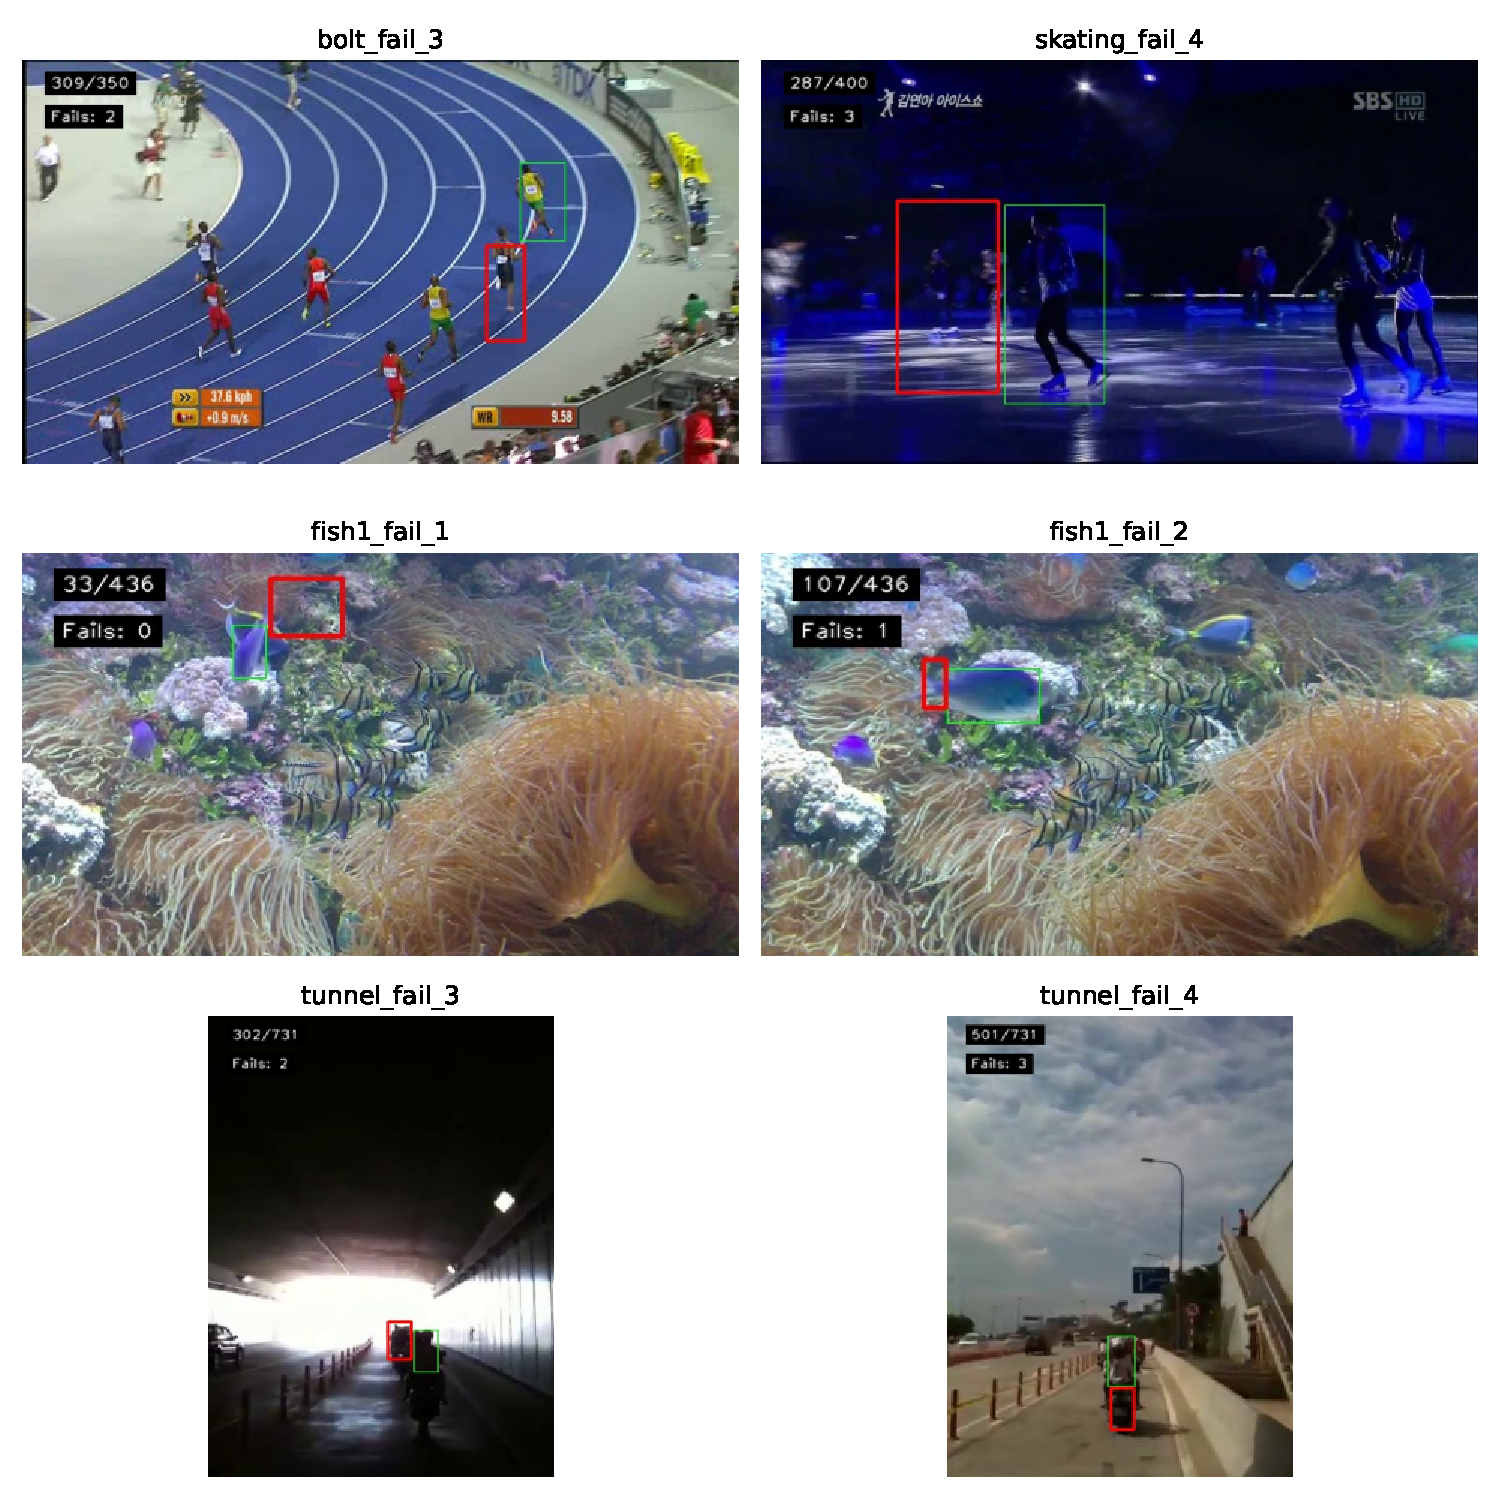
\includegraphics[width=1\columnwidth]{failures.pdf}
    \caption{Failure cases of the mean shift tracking algorithm.}
    \label{fig:failures}
\end{figure}

For the bolt sequence, the tracker fails because the object (Bolt) changes direction, moves fast and changes shape.
Increasing the kernel size could help with the fast moving object, but the shape change is a limitation of the mean shift algorithm.
In the skating sequence the lighting conditions change and the skater becomes darker then before, which leads to the tracker failing.
For the fish1 sequence the fish drastically changes shape and also moves in a fast jerking way.
To improve tracking in this case a larger update rate $\alpha$ would help with the fast jerking movements.
In the tunnel sequence the light changes significantly.
The target object in the left image is completley black and also changes lane to the right causing the tracker to fail.
After some time the tracker adapts to the the darker object color, when the moped comes out of the tunnel and into the light the tracker still tracks dark regions and converges to the (darker) bottom of the moped.
To imporve tracking in this case using a different colorspace (like HSV) might help.


\subsection*{Parameter tuning}
As mentioned before we used optimal parameters for the mean shift tracking algorithm.
To find these parameters we performed a grid search over the following parameters:
\begin{itemize}
    \item Kernel size: 11, 15, 21, 31, 51
    \item Update rate $\alpha$: 0.01, 0.02, 0.05, 0.1
    \item $\epsilon$: 1e-6, 1e-7,1e-8, 1e-9, 1e-10
\end{itemize}
In table \ref{tab:parameters} we show the 10 best performing parameter tuples.
We can observe that all the results use an update rate of 0.01, which is sensible with the notion that the target object does not change significantly between frames.
All the teseted kernel sizes are present in the best performing parameters.
This can be explained by the fact that the target moves by a small amount between frames and thus the mean shift starts near the maximum of the PDF.
Because of this, kernel sizes 11 and 15 are sufficient to converge to the target.
A similar observation can be made for the $\epsilon$ parameter, where the best performing values are in the range of 1e-7 to 1e-10.
For other tested parameter values the tracker quality is mostly dependant on the update rate $\alpha$.
As we increase the update rate, the number of errors increases significantly, this would be expected as the tracker would be more sensitive to changes in the target object.
\begin{table}[!ht]
    \centering
    \begin{tabular}{|lll||l|l|}
    \hline
        Kernel Size & Update Rate & Epsilon & Errors & FPS \\ \hline
        11 & 0.01 & 1e-7 & 42 & 756 \\ 
        11 & 0.01 & 1e-9 & 42 & 747 \\ 
        11 & 0.01 & 1e-6 & 42 & 731 \\ 
        11 & 0.01 & 1e-10 & 42 & 730 \\ 
        11 & 0.01 & 1e-8 & 42 & 722 \\ 
        51 & 0.01 & 1e-7 & 43 & 774 \\ 
        15 & 0.01 & 1e-7 & 43 & 751 \\ 
        31 & 0.01 & 1e-7 & 43 & 748 \\ 
        31 & 0.01 & 1e-9 & 43 & 745 \\ 
        21 & 0.01 & 1e-6 & 43 & 743 \\ \hline
    \end{tabular}
    \caption{Best performing parameters for the mean shift tracking algorithm.}
    \label{tab:parameters}
\end{table}



\section{Conclusion}
The limitations of the Mean Shift tracking algorithm can be seen in the failure cases.
The algorithm is not robust to fast moving objects, changes in lighting conditions and changes in object shape.
To improve the tracking a method to adapt size changes and adapt for light changes would need to be added.



\bibliographystyle{IEEEtran}
\bibliography{bibliography}

\end{document}
